\PassOptionsToPackage{table}{xcolor}
\documentclass[10pt]{beamer}
\usepackage[english]{babel}

% Beamer theme
\usetheme{metropolis}

\usepackage{smartdiagram}
\usepackage{lstautogobble}
\usepackage{listings}
\usepackage{booktabs}
\usepackage[scale=2]{ccicons}%creative commons
\setbeamercovered{transparent}%invisible by default
\usepackage{array}
\newcolumntype{L}[1]{>{\raggedright\let\newline\\arraybackslash\hspace{0pt}}m{#1}}
\newcolumntype{C}[1]{>{\centering\let\newline\\arraybackslash\hspace{0pt}}m{#1}}
\newcolumntype{R}[1]{>{\raggedleft\let\newline\\arraybackslash\hspace{0pt}}m{#1}}

\usepackage{pgfplots}
\usepgfplotslibrary{dateplot}
\usepackage{tikz}
\usetikzlibrary{positioning,chains,fit,shapes,calc}
\usetikzlibrary{positioning,chains,fit,shapes,calc,automata,positioning}
\usepackage{fancyvrb}

% To include metapost files.
\usepackage{ifpdf}                        % To check if pdflatex is used.
\ifpdf
  \DeclareGraphicsRule{*}{mps}{*}{}
\fi

% Define path for images.
\graphicspath{{./}, {./Images/}}

% few useful commands
\providecommand{\ie}{i.\,e.}
\providecommand{\Ie}{I.\,e.}
\providecommand{\eg}{e.\,g.}
\providecommand{\Eg}{E.\,g.}

% Basic listing setting (eg, autogobble to remove left margin)
\lstset{basicstyle=\ttfamily, autogobble}

% metropolis template settings
\metroset{block=fill}
\metroset{titleformat frame=smallcaps}

\title{Functional design of a simple board game}
%\subtitle{}

\date{\today}
\author[Alessandro Candolini]{Alessandro Candolini}
%\institute{}
% \titlegraphic{\hfill\includegraphics[height=1.5cm]{logo/logo}}

\begin{document}

\maketitle

\begin{frame}{Agenda}
  \setbeamertemplate{section in toc}[sections numbered]
  \tableofcontents[hideallsubsections]
\end{frame}

\section{Warm up}
\begin{frame}[fragile]
  \begin{figure}
    \centering
  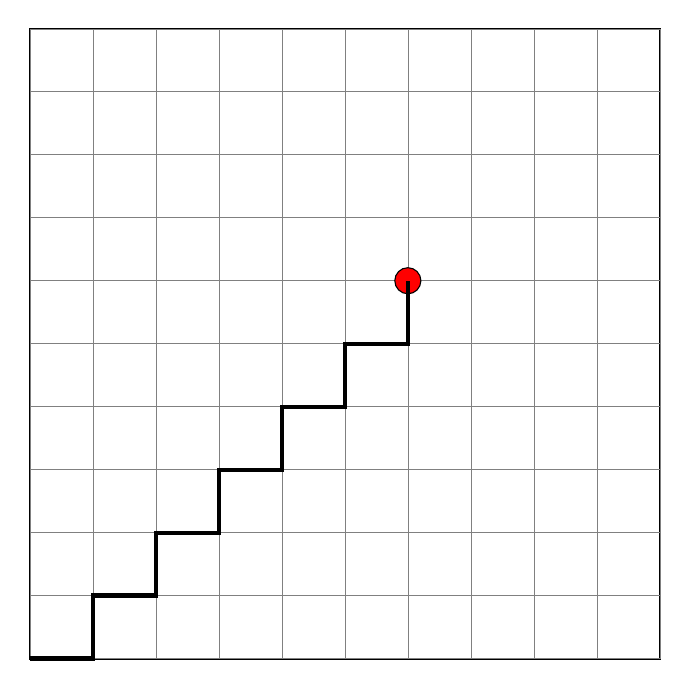
\begin{tikzpicture}[scale=0.8]
    % Draw board border
    \draw[thick] (0,0) rectangle (10,10);

    % Draw grid lines
    \draw[step=1cm,gray,very thin] (0,0) grid (10,10);

    % Draw food
    \node[draw,circle,fill=red] at (6,6) {};

    % Draw snake
    \draw[ultra thick] (0,0) -- (1,0) -- (1,1) -- (2,1) -- (2,2) -- (3,2) -- (3,3) -- (4,3) -- (4,4) -- (5,4) -- (5,5) -- (6,5) -- (6,6);
\end{tikzpicture}
  \end{figure}
\end{frame}

\begin{frame}[fragile]
  \begin{figure}
    \centering
  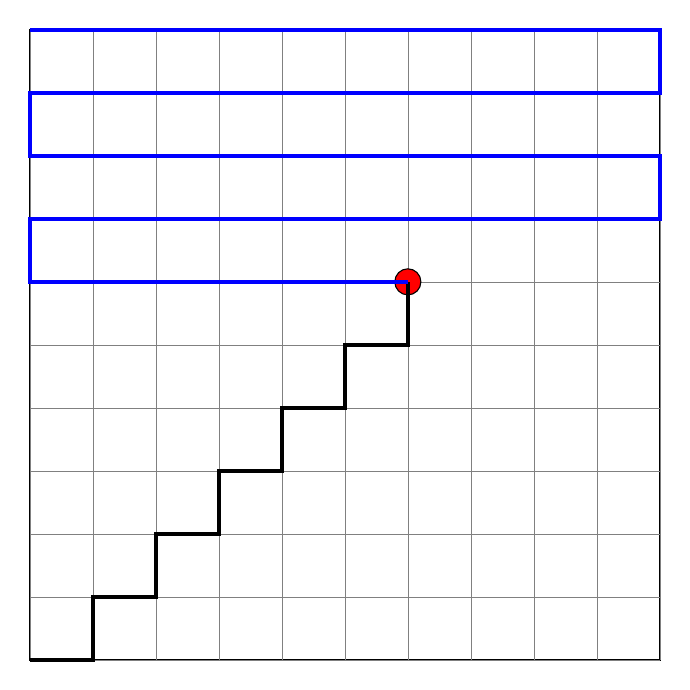
\begin{tikzpicture}[scale=0.8]
    % Draw board border
    \draw[thick] (0,0) rectangle (10,10);

    % Draw grid lines
    \draw[step=1cm,gray,very thin] (0,0) grid (10,10);

    % Draw food
    \node[draw,circle,fill=red] at (6,6) {};

    % Draw snake
    \draw[ultra thick] (0,0) -- (1,0) -- (1,1) -- (2,1) -- (2,2) -- (3,2) -- (3,3) -- (4,3) -- (4,4) -- (5,4) -- (5,5) -- (6,5) -- (6,6);
    % Draw snake2
    \draw[ultra thick, blue] (0, 10) -- (10, 10) -- (10, 9) -- (0, 9) -- (0,8) -- (10,8) -- (10, 7) -- (0, 7) -- (0, 6) -- (6, 6);
\end{tikzpicture}
  \end{figure}
\end{frame}

\begin{frame}[fragile]
  One strategy is described in words as follows:
  \begin{description}
      \item[] move right until the edge
      \item[then] move one step down
      \item[then] move left until the edge
      \item[then] move one step down
      \item[then] repeat
  \end{description}
\end{frame}
\begin{frame}[fragile]
  \begin{description}
      \item[] fill row right
      \item[and then] one step down
      \item[and then] fill row left
      \item[and then] one step down
  \end{description}
\end{frame}
\begin{frame}[fragile]
  \begin{description}
    \item[repeat]
    \item[]
      \begin{description}
      \item[] fill row right
      \item[and then] one step down
      \item[and then] fill row left
      \item[and then] one step down
  \end{description}
  \end{description}
\end{frame}

\begin{frame}[fragile]
\begin{lstlisting}[language=haskell, basicstyle=\ttfamily]
nextMoveH :: Position -> Maybe Move
nextMoveH (Pos x y) =
  if y `mod` 2 == 0 then
     (if x < 19 then
         Just RightM
      else (
         if y < 19 then Just DownM
         else Nothing)
     )
  else
     (if x > 0 then
         Just LeftM
      else (
         if y < 19 then Just DownM
      else Nothing)
     )
  \end{lstlisting}
\end{frame}
\begin{frame}[fragile]
\begin{lstlisting}[language=haskell, basicstyle=\ttfamily]
nextMoveH :: Int -> Position -> Maybe Move
nextMoveH n (Pos x y) =
  if y `mod` 2 == 0 then
     (if x < (n-1) then
         Just RightM
      else (
         if y < (n-1) then Just DownM
         else Nothing)
     )
  else
     (if x > 0 then
         Just LeftM
      else (
         if y < (n-1) then Just DownM
      else Nothing)
     )
  \end{lstlisting}
\end{frame}
\begin{frame}[fragile]
  \begin{columns}%[T]
\begin{column}{0.5\textwidth}
  \begin{figure}
    \includegraphics[width=\columnwidth]{jira}
  \end{figure}
        \end{column}
            \vrule{}
        \begin{column}{0.5\textwidth}
  \begin{figure}
    \includegraphics[width=\columnwidth]{code}
  \end{figure}
        \end{column}
   \end{columns}
\end{frame}

\begin{frame}[fragile]
  \begin{columns}%[T]
\begin{column}{0.5\textwidth}
      \begin{description}
      \item[] fill row right
      \item[and then] one step down
      \item[and then] fill row left
      \item[and then] one step down
  \end{description}
        \end{column}
            \vrule{}
        \begin{column}{0.5\textwidth}
\begin{lstlisting}[language=haskell, basicstyle=\ttfamily\footnotesize]
nextMoveH :: Int -> Position
   -> Maybe Move
nextMoveH n (Pos x y) =
  if y `mod` 2 == 0 then
     (if x < (n-1) then
         Just RightM
      else (
         if y < (n-1) then
           Just DownM
         else Nothing)
     )
  else
     (if x > 0 then
         Just LeftM
      else (
         if y < (n-1) then
           Just DownM
         else Nothing)
     )
  \end{lstlisting}
        \end{column}
            \end{columns}
\end{frame}

\begin{frame}[fragile]
\begin{itemize}
  \item hypersensitivity to details (eg, choice of coordinates)
  \item focus on \emph{operational} concerns (\ie, the \emph{how}) vs \emph{denotational} concerns (\ie, the \emph{what})
  \item impedence mismatch between acceptance criteria and implementation, obfuscating the aim / behaviour of the code (ie, need to reverse engineering the code to understand the requirements)
  \item lack of composability

\end{itemize}
\end{frame}

\begin{frame}[fragile]
\begin{description}
      \item[] fill right
      \item[and then] one step down
      \item[and then] fill left
      \item[and then] one step down
  \end{description}
\end{frame}
\begin{frame}[fragile]
\begin{description}
      \item[] fill right
      \item[andThen] oneStep down
      \item[andThen] fill left
      \item[andThen] oneStep down
  \end{description}
\end{frame}

\begin{frame}[fragile]
\begin{lstlisting}[language=haskell, basicstyle=\ttfamily]
horizontal = repeat $ fill right
   `andThen` oneStep down
   `andThen` fill left
   `andThen` oneStep down
\end{lstlisting}
\end{frame}

\begin{frame}[fragile]
\begin{lstlisting}[language=haskell, basicstyle=\ttfamily]
vertical = repeat $
   fill down
   `andThen` oneStep right
   `andThen` fill up
   `andThen` oneStep right
\end{lstlisting}
\end{frame}

\section{Algebra of moves}

\begin{frame}[fragile]
\begin{lstlisting}[language=haskell, basicstyle=\ttfamily]
import Prelude hiding (Right, Left)

data Direction = Left | Right | Up | Down
         deriving (Eq, Show, Enum, Bounded)

data Position = P Int Int deriving (Eq,Show)
\end{lstlisting}
\end{frame}
\begin{frame}[fragile]
\begin{lstlisting}[language=haskell, basicstyle=\ttfamily]
\end{lstlisting}
\end{frame}
\begin{frame}[fragile]
  \begin{lstlisting}[language=haskell, basicstyle=\ttfamily]
data Move

step :: Direction -> Move

runMove :: Move -> Position -> Position
\end{lstlisting}
\end{frame}
\begin{frame}[fragile]
\begin{lstlisting}[language=haskell, basicstyle=\ttfamily]
left = step Left
right = step Right
up = step Up
down = step Down

runMove left (P 1 1) `shouldBe` (P 0 1)
runMove right (P 1 1) `shouldBe` (P 2 1)
runMove up (P 1 1) `shouldBe` (P 1 2)
runMove up (P 1 1) `shouldBe` (P 1 0)
\end{lstlisting}
\end{frame}
\begin{frame}[fragile]
\begin{lstlisting}[language=haskell, basicstyle=\ttfamily]
data Move = Move {
   runMove :: Position -> Position }

\end{lstlisting}
\end{frame}
\begin{frame}[fragile]
\begin{lstlisting}[language=haskell, basicstyle=\ttfamily]
data Move = Step Direction
    derives (Eq, Show)
\end{lstlisting}
\end{frame}
\begin{frame}[fragile]
\begin{lstlisting}[language=haskell, basicstyle=\ttfamily]
upRight = up <> right 
twoUpOneRight = up <> up <> right 
\end{lstlisting}
\end{frame}
\begin{frame}[fragile]
\begin{lstlisting}[language=haskell, basicstyle=\ttfamily]
data Move = DontMove
    | Step Direction
    | Compose Move Move derives (Eq, Show)
  \end{lstlisting}
\end{frame}
\begin{frame}[fragile]
\begin{lstlisting}[language=haskell, basicstyle=\ttfamily]
instance Semigroup Move where
  m1 <> m2 = Compose m1 m2

instance Monoid Move where
  mempty = DontMove
\end{lstlisting}
\end{frame}
\begin{frame}[fragile]
\begin{lstlisting}[language=haskell, basicstyle=\ttfamily]
{-# LANGUAGE DerivingVia #-}

newtype Move = Move  {
   endo :: Endo Position } deriving
     (Semigroup, Monoid) via (Endo Position)

runMove :: Move -> Position -> Position
runMove = appEndo . endo

\end{lstlisting}
\end{frame}
\begin{frame}[fragile]
\begin{lstlisting}[language=haskell, basicstyle=\ttfamily]
simplify :: Move -> Move 
simplify DontMove = DontMove 
simplify s@(Step d) = s
simplify (Compose m1 m2) = 
  case (simplify m1, simplify m2) of 
   (DontMove, m) -> m 
   (m, DontMove) -> m 
   (Step Left, Step Right) -> DontMove
   (Step Right, Step Left) -> DontMove
   (p1, p2) -> Compose p1 p2
\end{lstlisting}

  Notice:  This implementation does not take into account associativity
\end{frame}


\begin{frame}[fragile]
\begin{lstlisting}[language=haskell, basicstyle=\ttfamily]
instance Group Move where
  invert Stay = Stay
  invert (Step Right) = Step Left
  invert (Step Left) = Step Right
  invert (Step Up) = Step Down
  invert (Step Down) = Step Up
  invert (Combine m1 m2) = 
    Combine (invert m2) (invert m1)
\end{lstlisting}
\end{frame}

\section{Algebra of strategies}

\begin{frame}[fragile]
\begin{lstlisting}[language=haskell, basicstyle=\ttfamily]

data Board 

rectangular :: Int -> Int -> Board 

square n = rectangular n n 

data Availability = Available | Unavailable
   deriving (Eq,Show)

check :: Board -> Position -> Availability 

\end{lstlisting}
\end{frame}

\begin{frame}[fragile]
\begin{lstlisting}[language=haskell, basicstyle=\ttfamily]
data Board = Board { 
   check :: Position -> Availability } 
\end{lstlisting}
\end{frame}
\begin{frame}[fragile]
\begin{lstlisting}[language=haskell, basicstyle=\ttfamily]
data Board = SquareBoard Int
   deriving (Eq,Show) 

check (SquareBoard n) (P x y) = undefined

draw :: Board -> Text
\end{lstlisting}
\end{frame}
\begin{frame}[fragile]
\begin{lstlisting}[language=haskell, basicstyle=\ttfamily]
data Strategy 

oneStep :: Move -> Strategty 
andThen :: Strategy -> Strategy -> Strategy 

run :: Strategy -> Board -> Position -> [Position]
\end{lstlisting}
\end{frame}
\begin{frame}[fragile]
\begin{lstlisting}[language=haskell, basicstyle=\ttfamily]
s = oneStep right `andThen` oneStep down
\end{lstlisting}
\end{frame}
\begin{frame}[fragile]
  \begin{lstlisting}[language=haskell, basicstyle=\ttfamily]
  \end{lstlisting}
\end{frame}
\begin{frame}[fragile]
  \begin{lstlisting}[language=haskell, basicstyle=\ttfamily]
  \end{lstlisting}
\end{frame}
\begin{frame}[fragile]
  \begin{lstlisting}[language=haskell, basicstyle=\ttfamily]
  \end{lstlisting}
\end{frame}
\begin{frame}[fragile]
  \begin{lstlisting}[language=haskell, basicstyle=\ttfamily]
  \end{lstlisting}
\end{frame}
\begin{frame}[fragile]
  \begin{lstlisting}[language=haskell, basicstyle=\ttfamily]
  \end{lstlisting}
\end{frame}
\begin{frame}[fragile]
  \begin{lstlisting}[language=haskell, basicstyle=\ttfamily]
  \end{lstlisting}
\end{frame}
\begin{frame}[fragile]
  \begin{lstlisting}[language=haskell, basicstyle=\ttfamily]
  \end{lstlisting}
\end{frame}
\begin{frame}[fragile]
  \begin{lstlisting}[language=haskell, basicstyle=\ttfamily]
  \end{lstlisting}
\end{frame}
\begin{frame}[fragile]
  \begin{lstlisting}[language=haskell, basicstyle=\ttfamily]
  \end{lstlisting}
\end{frame}
\begin{frame}[fragile]
  \begin{lstlisting}[language=haskell, basicstyle=\ttfamily]
  \end{lstlisting}
\end{frame}
\begin{frame}[fragile]
  \begin{lstlisting}[language=haskell, basicstyle=\ttfamily]
  \end{lstlisting}
\end{frame}
\begin{frame}[fragile]
  \begin{lstlisting}[language=haskell, basicstyle=\ttfamily]
  \end{lstlisting}
\end{frame}
\begin{frame}[fragile]
  \begin{lstlisting}[language=haskell, basicstyle=\ttfamily]
  \end{lstlisting}
\end{frame}
\begin{frame}[fragile]
  \begin{lstlisting}[language=haskell, basicstyle=\ttfamily]
  \end{lstlisting}
\end{frame}
\begin{frame}[fragile]
  \begin{lstlisting}[language=haskell, basicstyle=\ttfamily]
  \end{lstlisting}
\end{frame}
\begin{frame}[fragile]
  \begin{lstlisting}[language=haskell, basicstyle=\ttfamily]
  \end{lstlisting}
\end{frame}
\begin{frame}[fragile]
  \begin{lstlisting}[language=haskell, basicstyle=\ttfamily]
  \end{lstlisting}
\end{frame}
\begin{frame}[fragile]
  \begin{lstlisting}[language=haskell, basicstyle=\ttfamily]
  \end{lstlisting}
\end{frame}
\begin{frame}[fragile]
  \begin{lstlisting}[language=haskell, basicstyle=\ttfamily]
  \end{lstlisting}
\end{frame}
\begin{frame}[fragile]
  \begin{lstlisting}[language=haskell, basicstyle=\ttfamily]
  \end{lstlisting}
\end{frame}
\begin{frame}[fragile]
  \begin{lstlisting}[language=haskell, basicstyle=\ttfamily]
  \end{lstlisting}
\end{frame}


\section{Advanced considerations}
\begin{frame}[fragile]
  \begin{itemize}
    \item random generation
    \item walls
    \item self avoiding (single player)
    \item self avoiding (multiplayer)
    \item UI + latex output
  \end{itemize}
\end{frame}
\plain{Questions?}

%\begin{frame}[allowframebreaks] {References}
% \bibliography{demo}
% \bibliographystyle{abbrv}
%\end{frame}

\end{document}
%% Useful for copy pasting. Would be better to just have snippets
\begin{frame}[fragile]
  \begin{lstlisting}[language=haskell, basicstyle=\ttfamily]
  \end{lstlisting}
\end{frame}
\begin{frame}[fragile]
  \frametitle{}
  \begin{lstlisting}[language=haskell, basicstyle=\ttfamily]
  \end{lstlisting}
\end{frame}
